\chapter{Исследовательская часть}

Для тестирования разработанного алгоритма применялась облачная платформа Google Colab, не требующая установки ПО на локальный компьютер.

\section{Агломеративная кластеризация}

\subsection{Кластеризация исходных данных}

\begin{figure}
	\begin{center}
		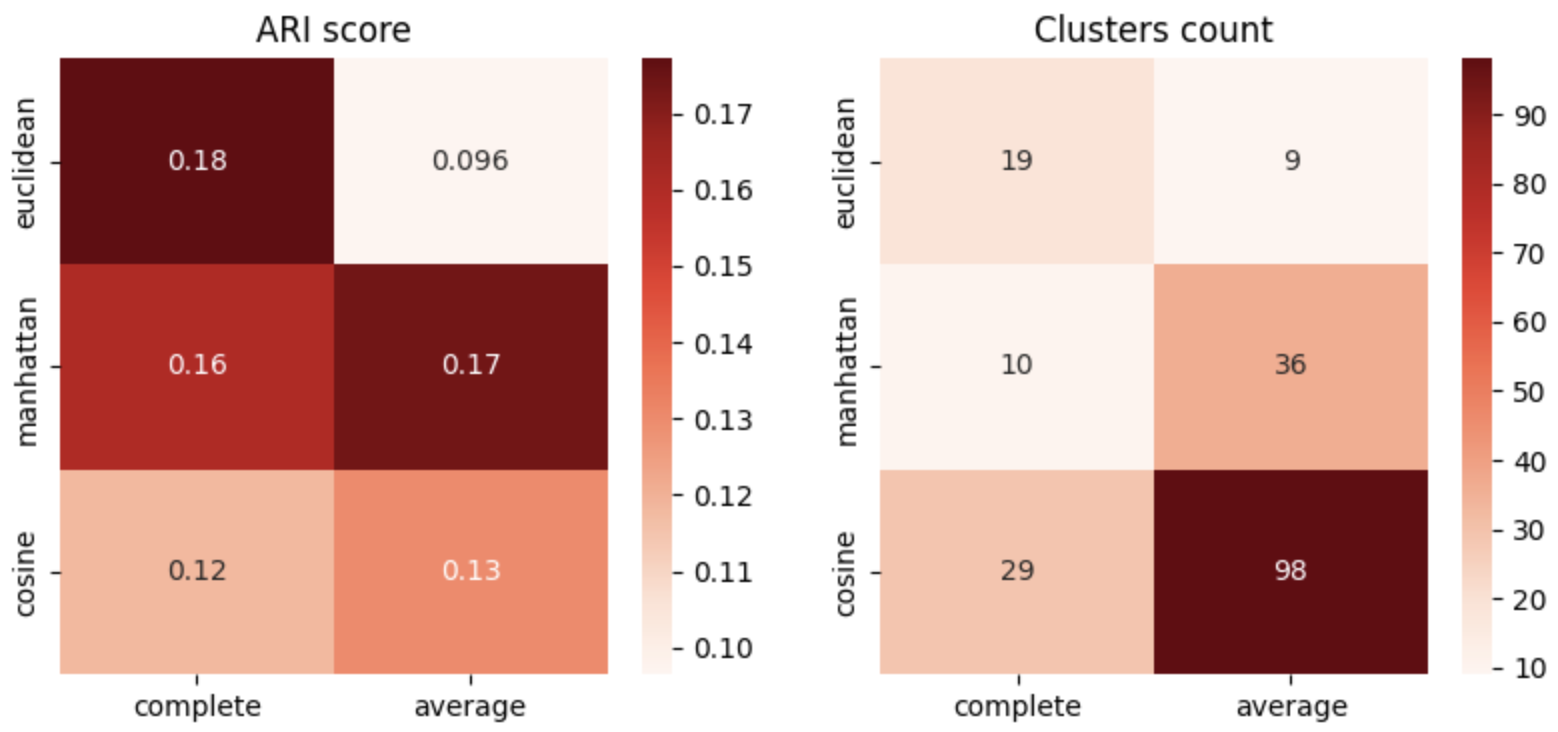
\includegraphics[width=\textwidth]{images/1.png}
	\end{center}
	\caption{Сравнение метрик при использовании различных расстояний и критериев связи в алгоритме агломеративной кластеризации исходных данных}
	\label{img:1}
\end{figure}

\begin{figure}
	\begin{center}
		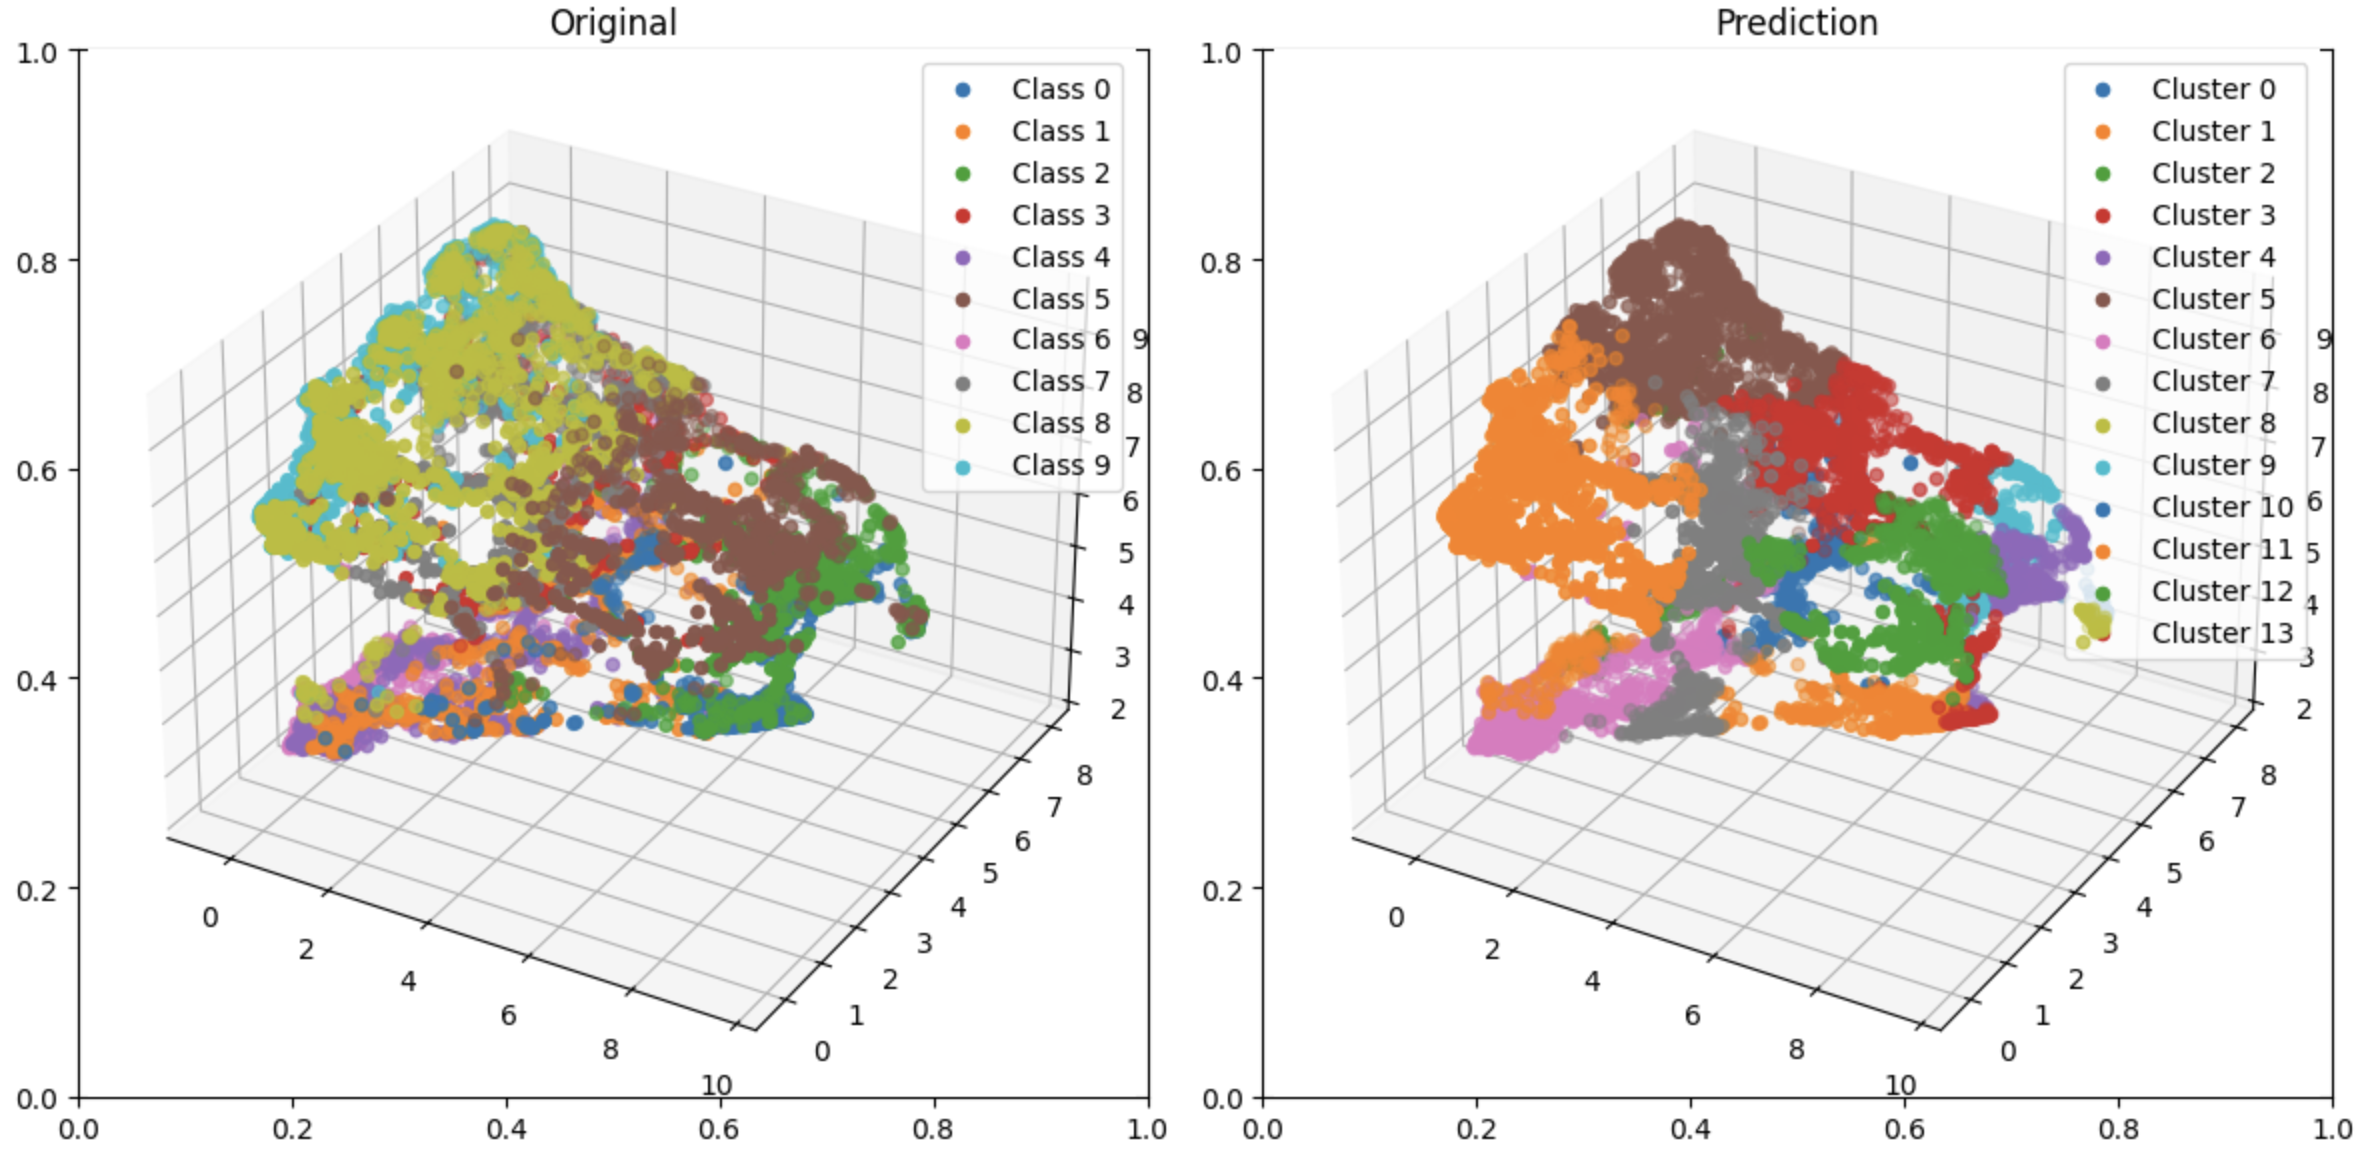
\includegraphics[width=\textwidth]{images/2.png}
	\end{center}
	\caption{Сравнение оригинального разбиения респондентов по шкале Кантрила с результатом кластеризации исходных данных (ARI: 0.18)}
	\label{img:2}
\end{figure}

\begin{figure}
	\begin{center}
		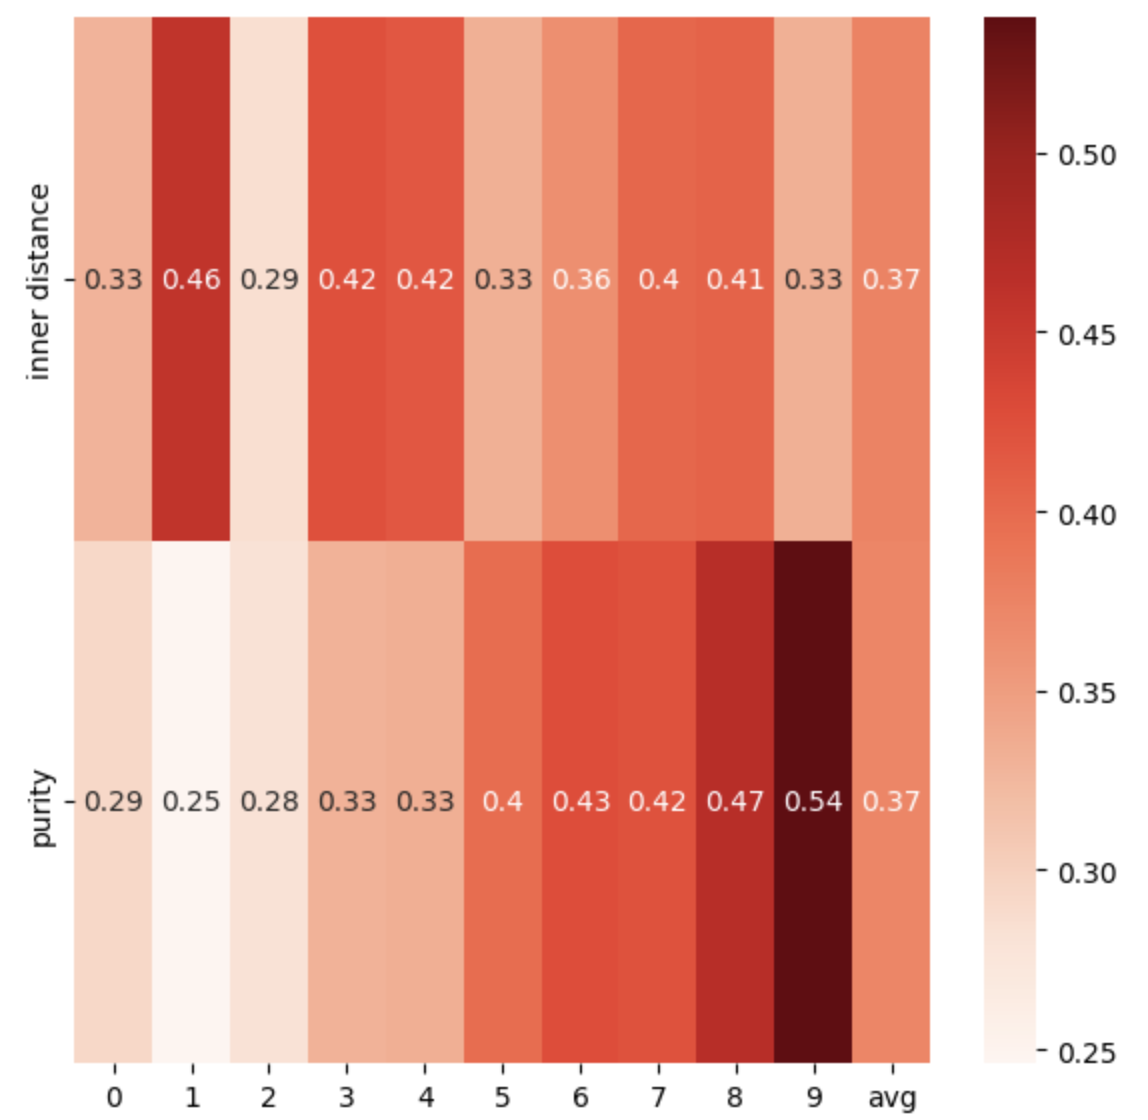
\includegraphics[width=0.6\textwidth]{images/4.png}
	\end{center}
	\caption{Соотнесение внутрикластерных расстояний с чистотой исходных кластеров, отсортированных по шкале Кантрила)}
	\label{img:3}
\end{figure}

\FloatBarrier

\subsection{Кластеризация векторов, полученных после снижения размерности исходных данных с помощью алгоритма UMAP}

\begin{figure}
	\begin{center}
		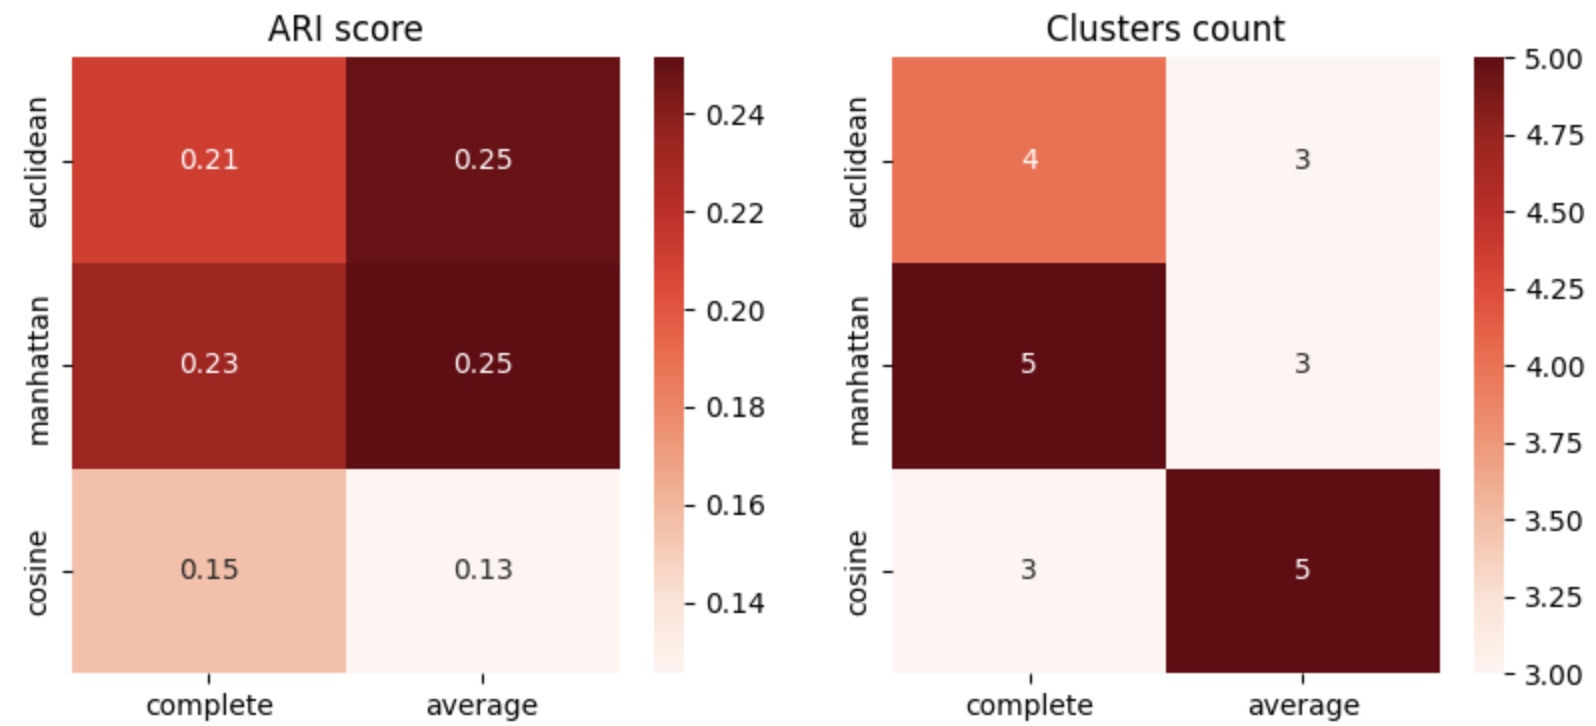
\includegraphics[width=\textwidth]{images/5.png}
	\end{center}
	\caption{Сравнение метрик при использовании различных расстояний и критериев связи в алгоритме агломеративной кластеризации векторов, полученных после снижения размерности исходных данных с помощью алгоритма UMAP}
	\label{img:4}
\end{figure}

\begin{figure}
	\begin{center}
		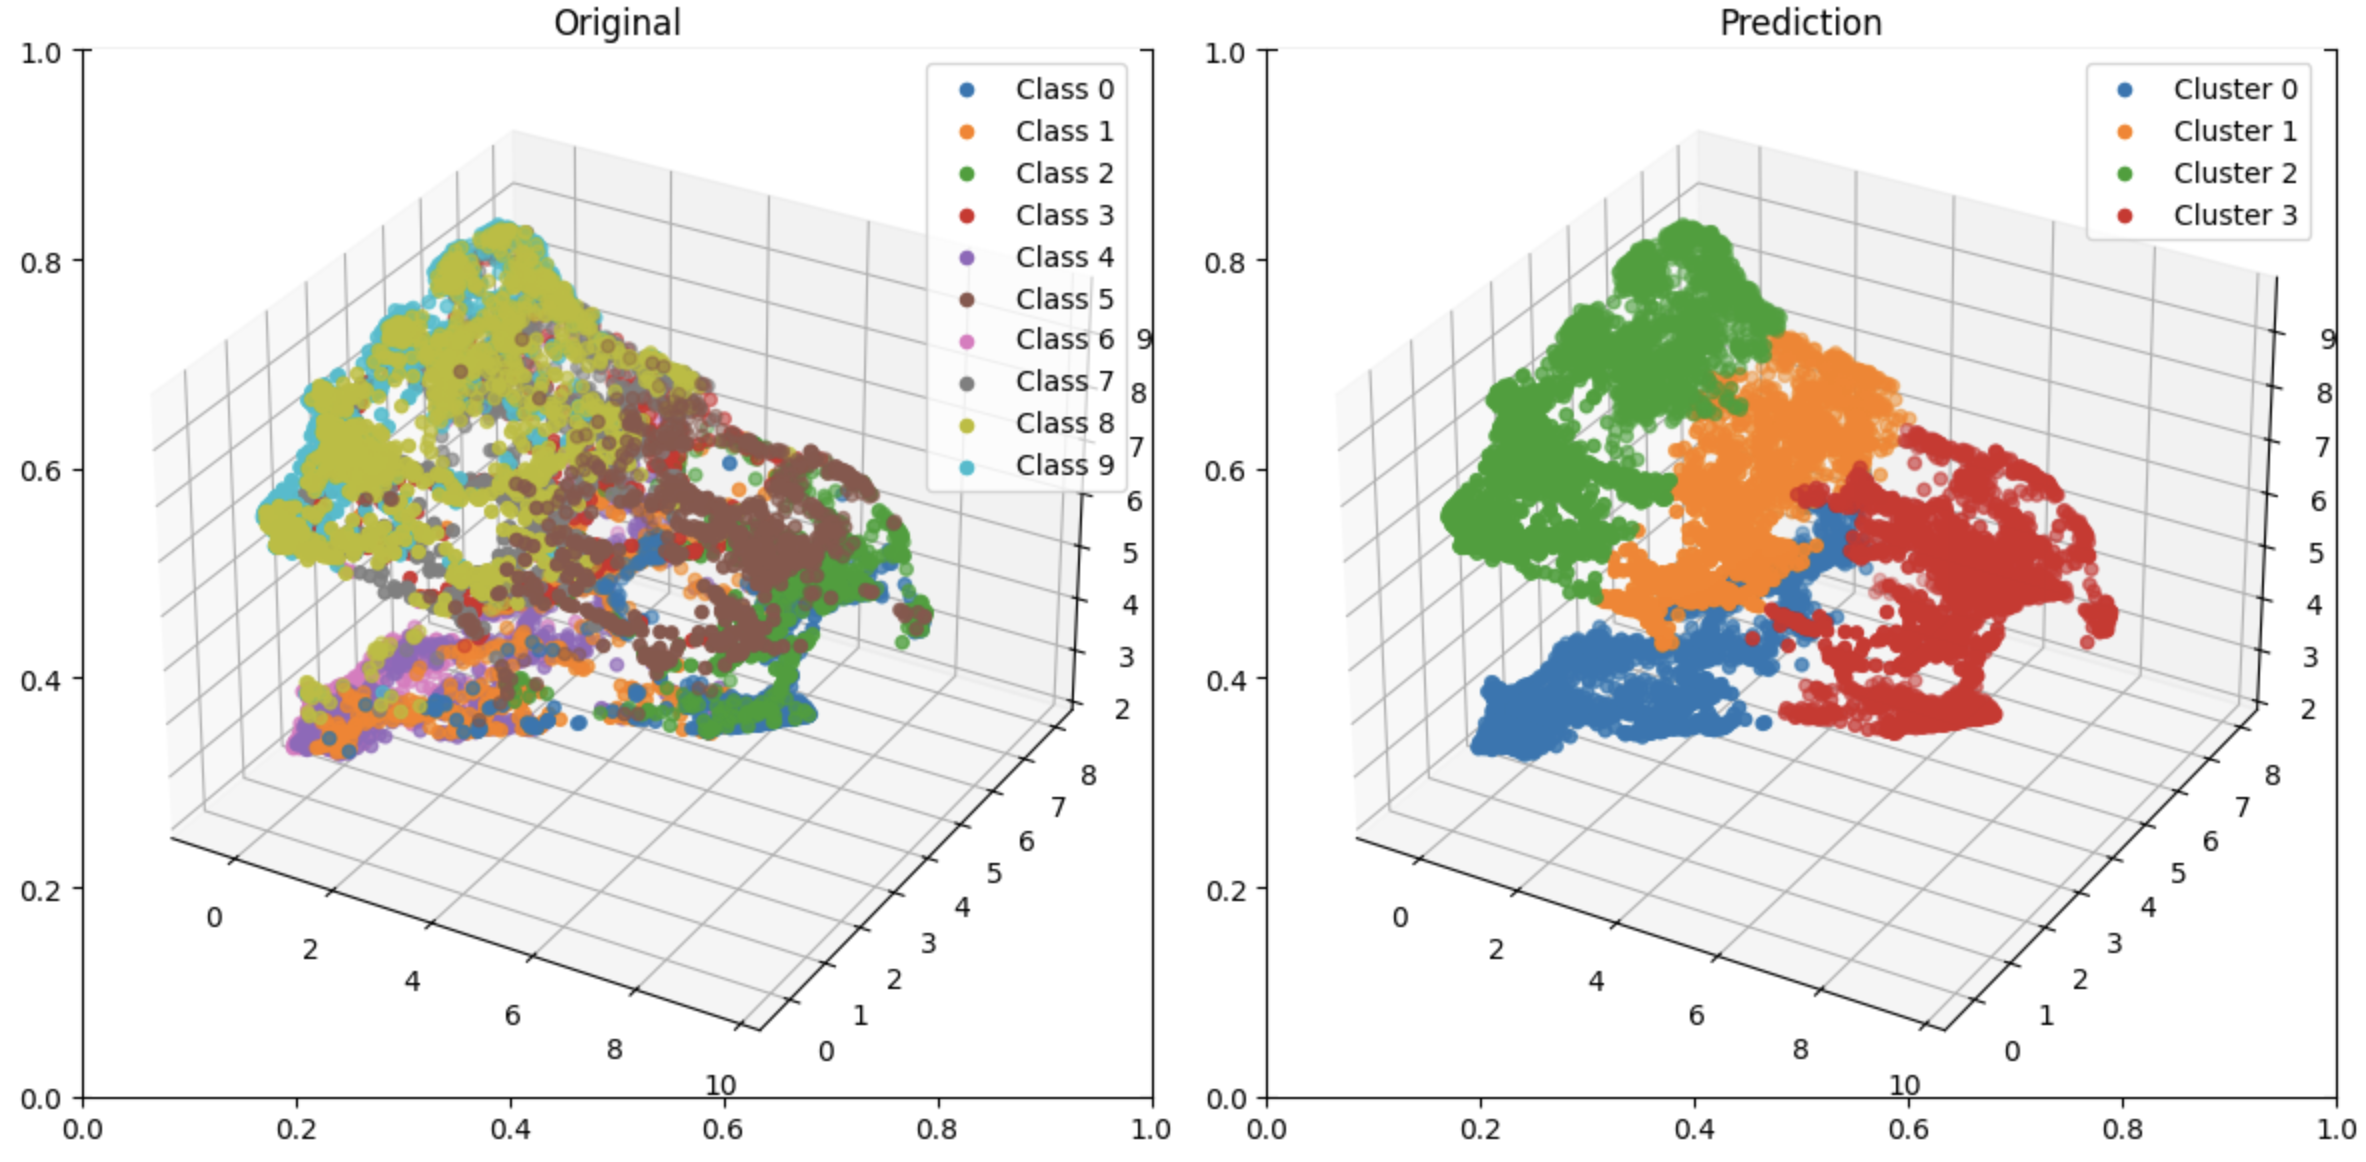
\includegraphics[width=\textwidth]{images/6.png}
	\end{center}
	\caption{Сравнение оригинального разбиения респондентов по шкале Кантрила с результатом кластеризации исходных данных (ARI: 0.27)}
	\label{img:5}
\end{figure}

\begin{figure}
	\begin{center}
		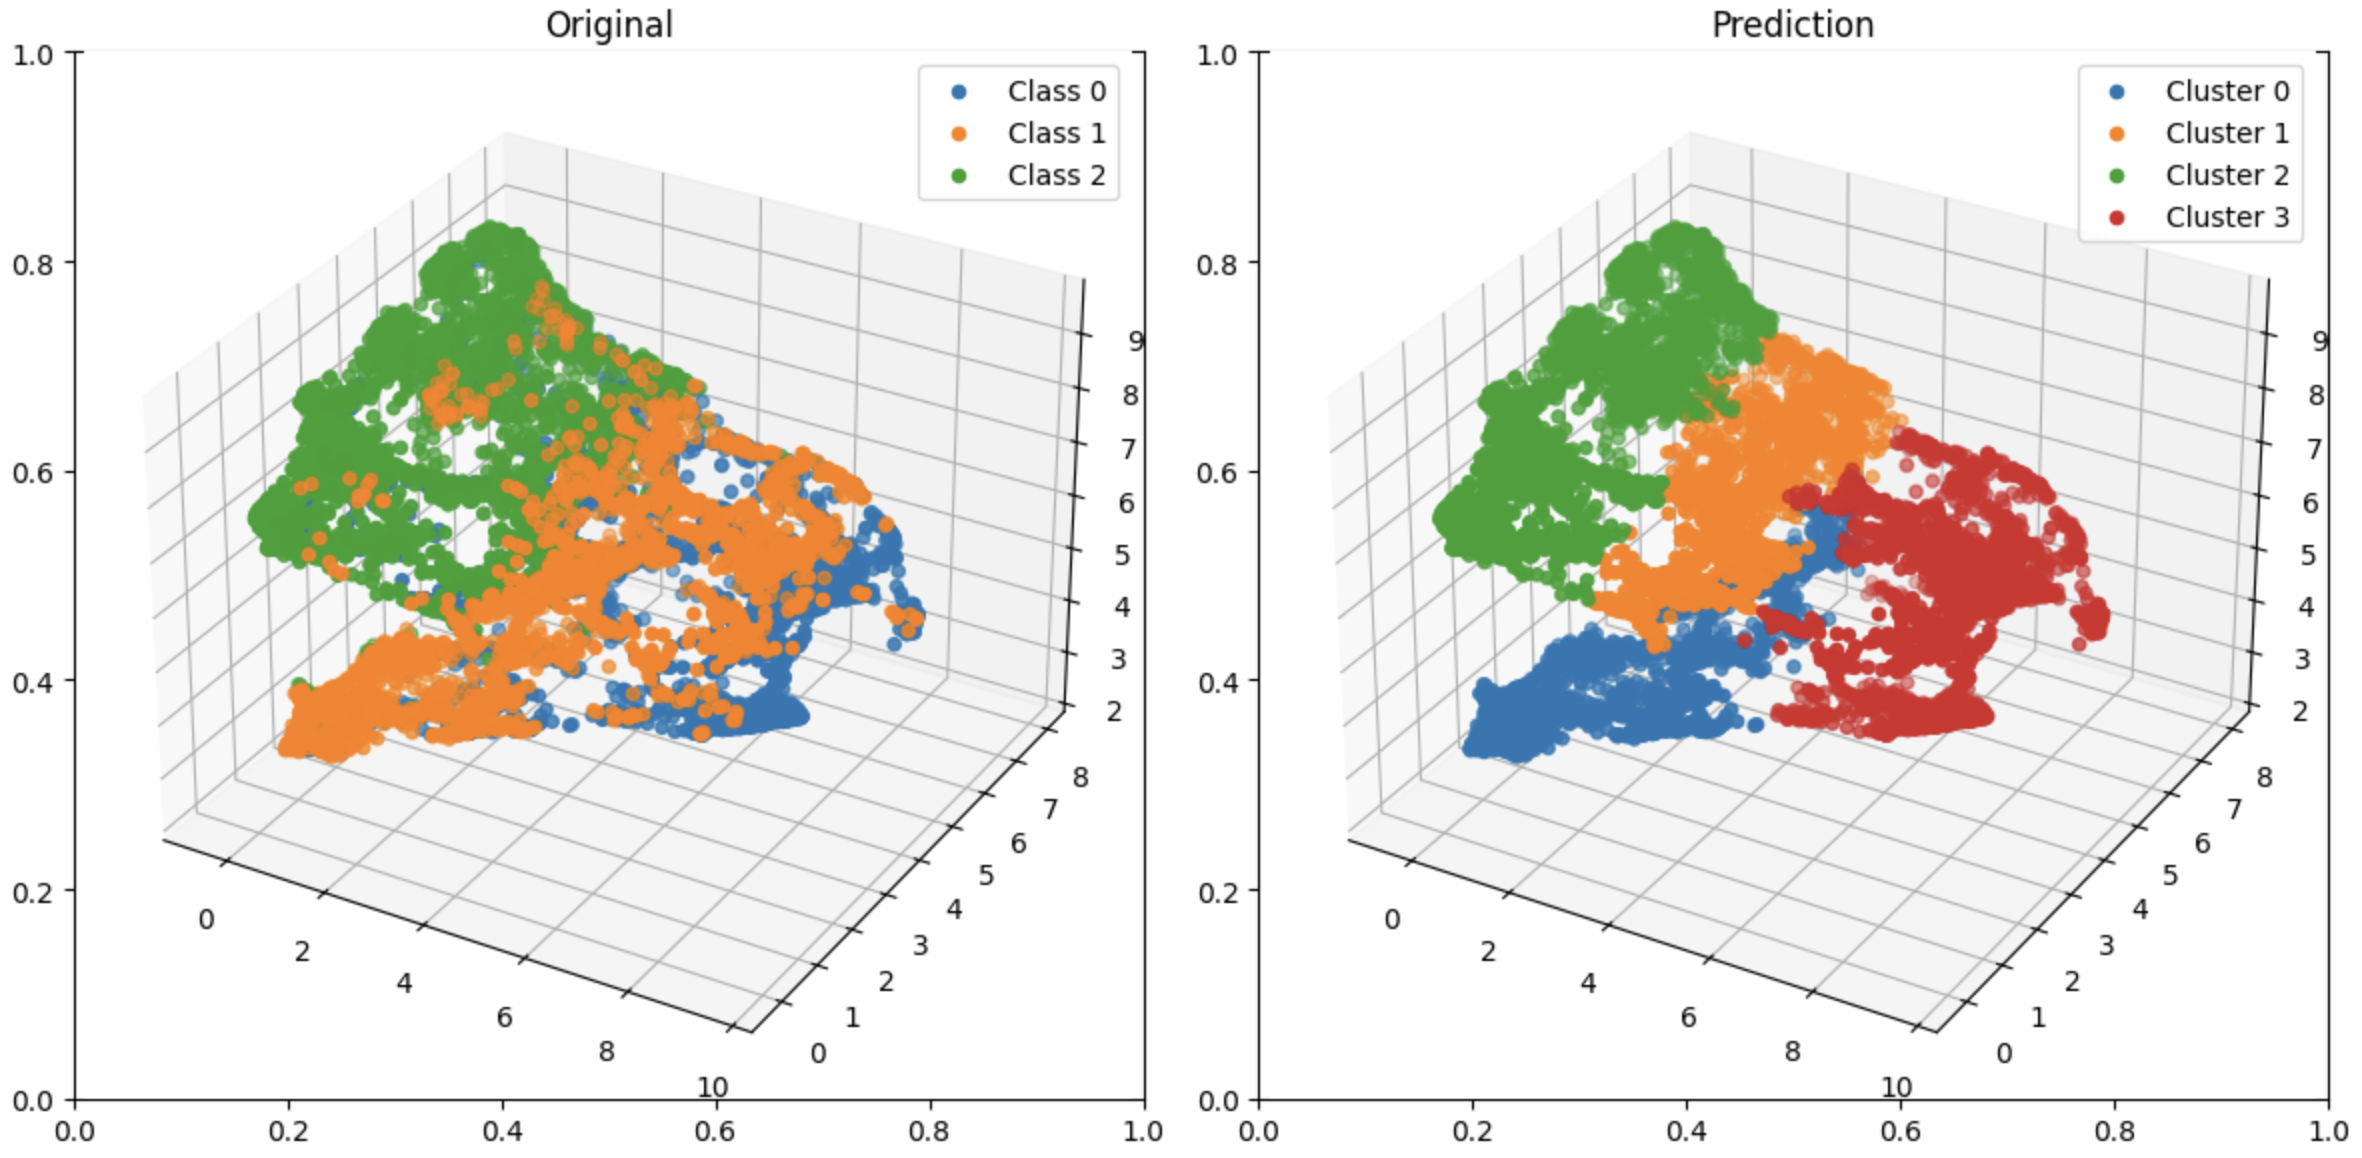
\includegraphics[width=\textwidth]{images/7.png}
	\end{center}
	\caption{Сравнение оригинального разбиения респондентов по укрупнённой шкале Кантрила с результатом кластеризации исходных данных (ARI: 0.37)}
	\label{img:6}
\end{figure}

\begin{figure}
	\begin{center}
		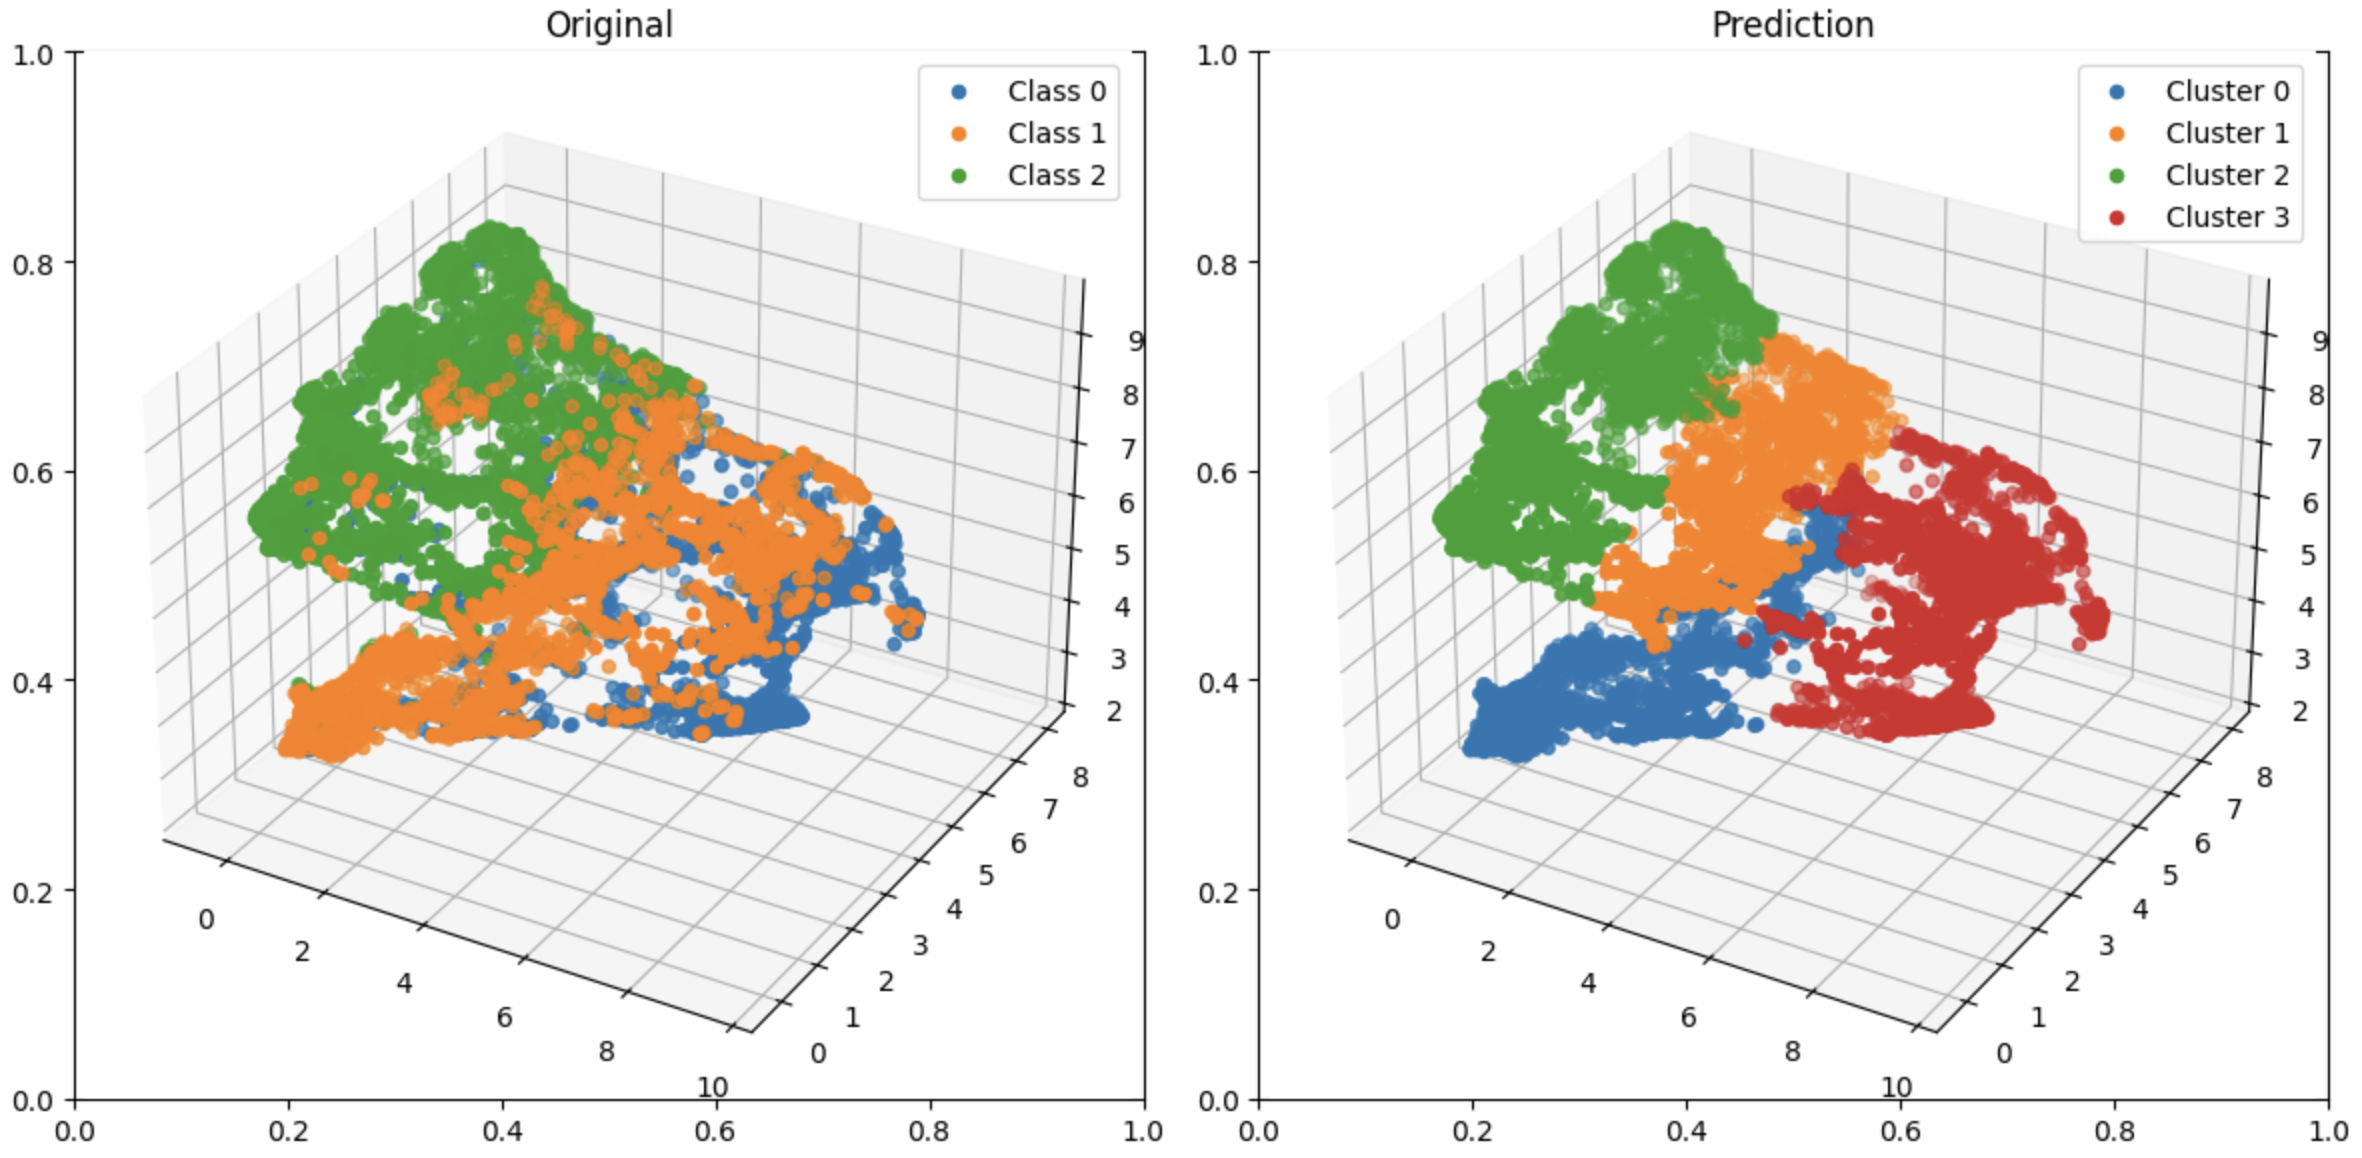
\includegraphics[width=\textwidth]{images/7.png}
	\end{center}
	\caption{Соотнесение внутрикластерных расстояний с чистотой исходных кластеров, отсортированных по укрупнённой шкале Кантрила)}
	\label{img:7}
\end{figure}

\FloatBarrier

\subsection{Подбор количества кластеров}

\begin{figure}
	\begin{center}
		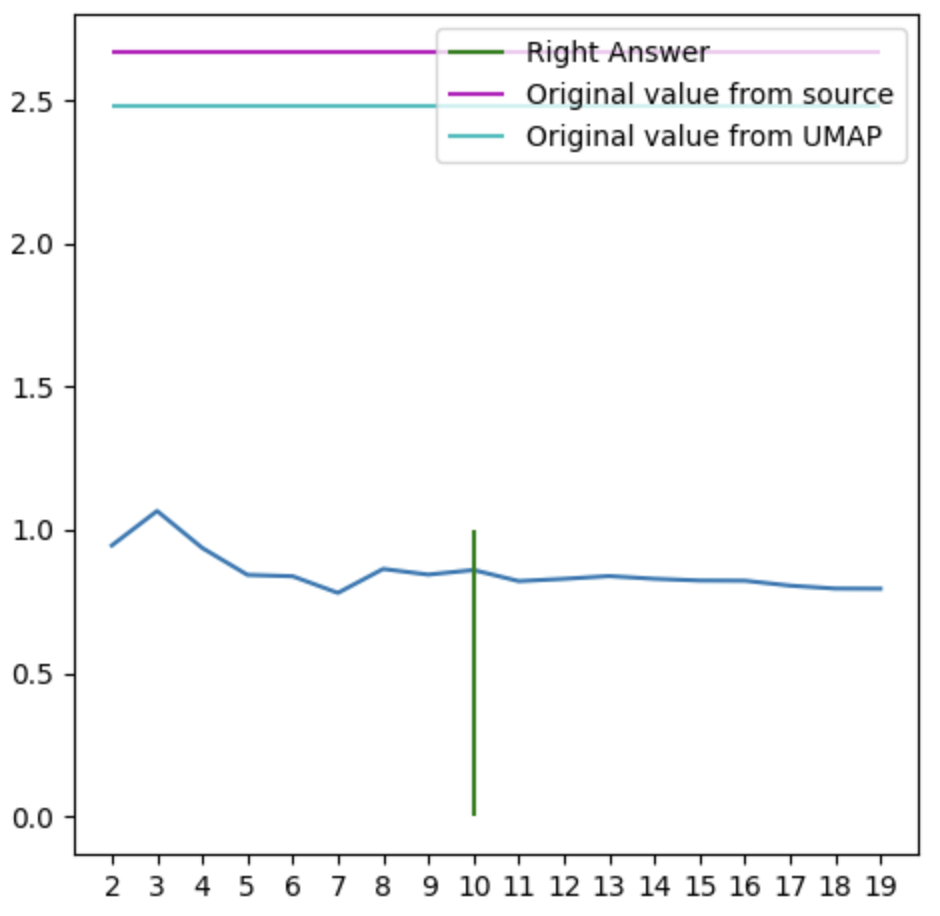
\includegraphics[width=0.6\textwidth]{images/10.png}
	\end{center}
	\caption{Зависимость метрики DBI от заданного количества кластеров}
	\label{img:8}
\end{figure}

\begin{figure}
	\begin{center}
		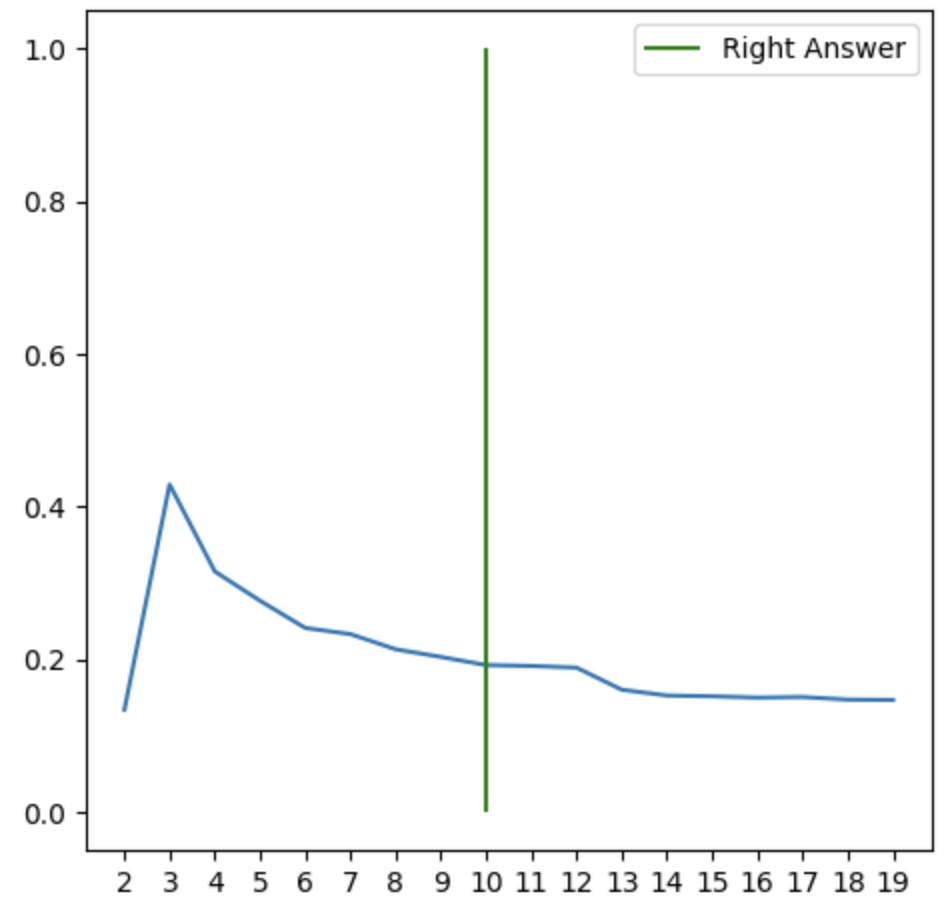
\includegraphics[width=0.6\textwidth]{images/11.png}
	\end{center}
	\caption{Зависимость метрики ARI от заданного количества кластеров}
	\label{img:9}
\end{figure}

\begin{figure}
	\begin{center}
		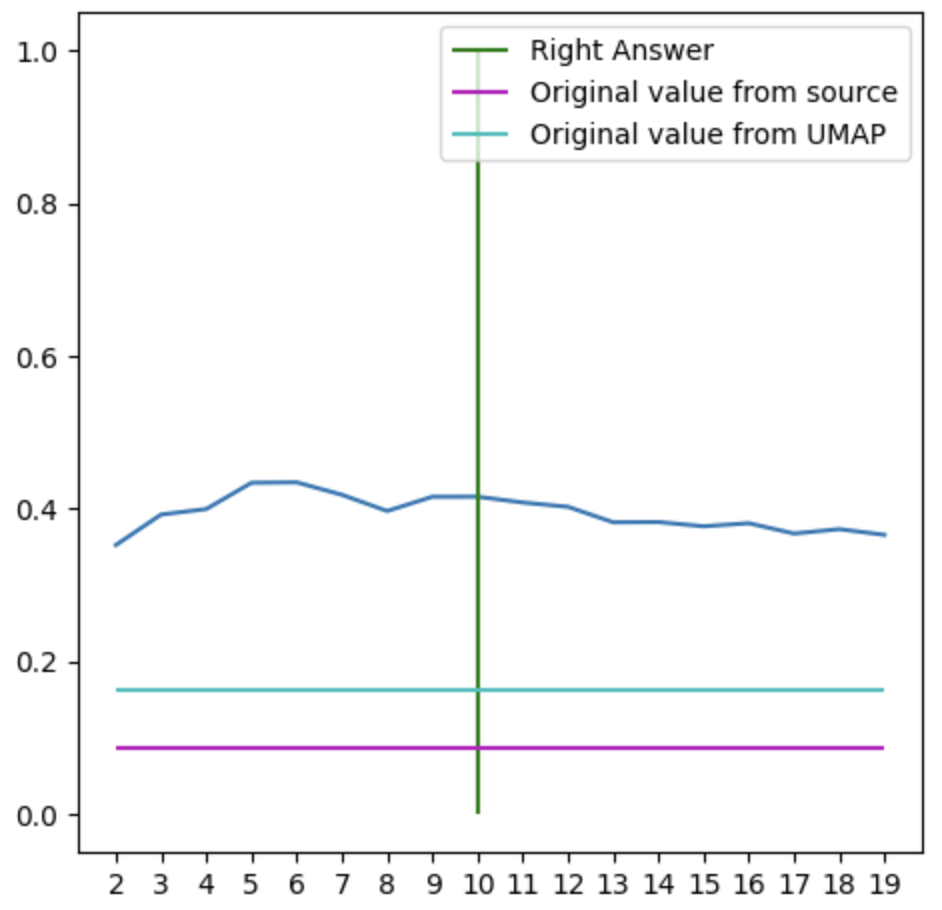
\includegraphics[width=0.6\textwidth]{images/12.png}
	\end{center}
	\caption{Зависимость метрики Silhouette score от заданного количества кластеров}
	\label{img:10}
\end{figure}

\begin{figure}
	\begin{center}
		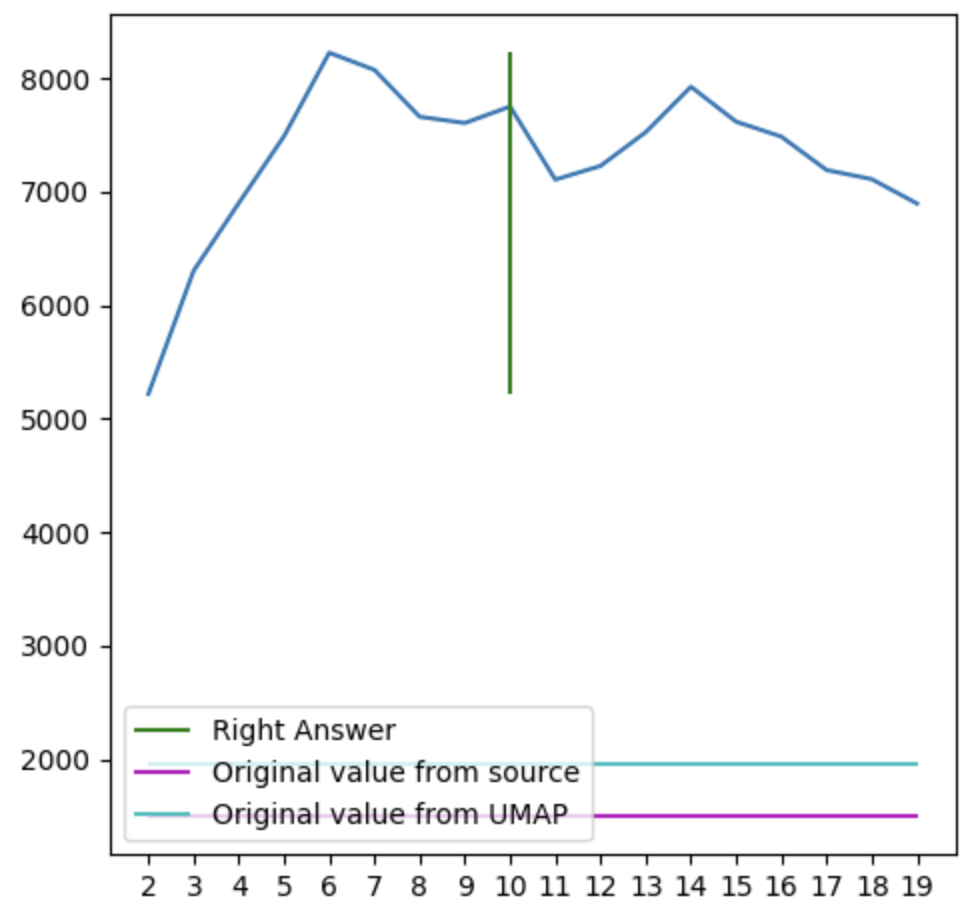
\includegraphics[width=0.6\textwidth]{images/13.png}
	\end{center}
	\caption{Зависимость метрики Calinski Harabasz score от заданного количества кластеров}
	\label{img:11}
\end{figure}

\FloatBarrier

\section{Алгоритм HDBSCAN}

\subsection{Оптимизация гиперпараметров по метрике ARI}

\begin{figure}
	\begin{center}
		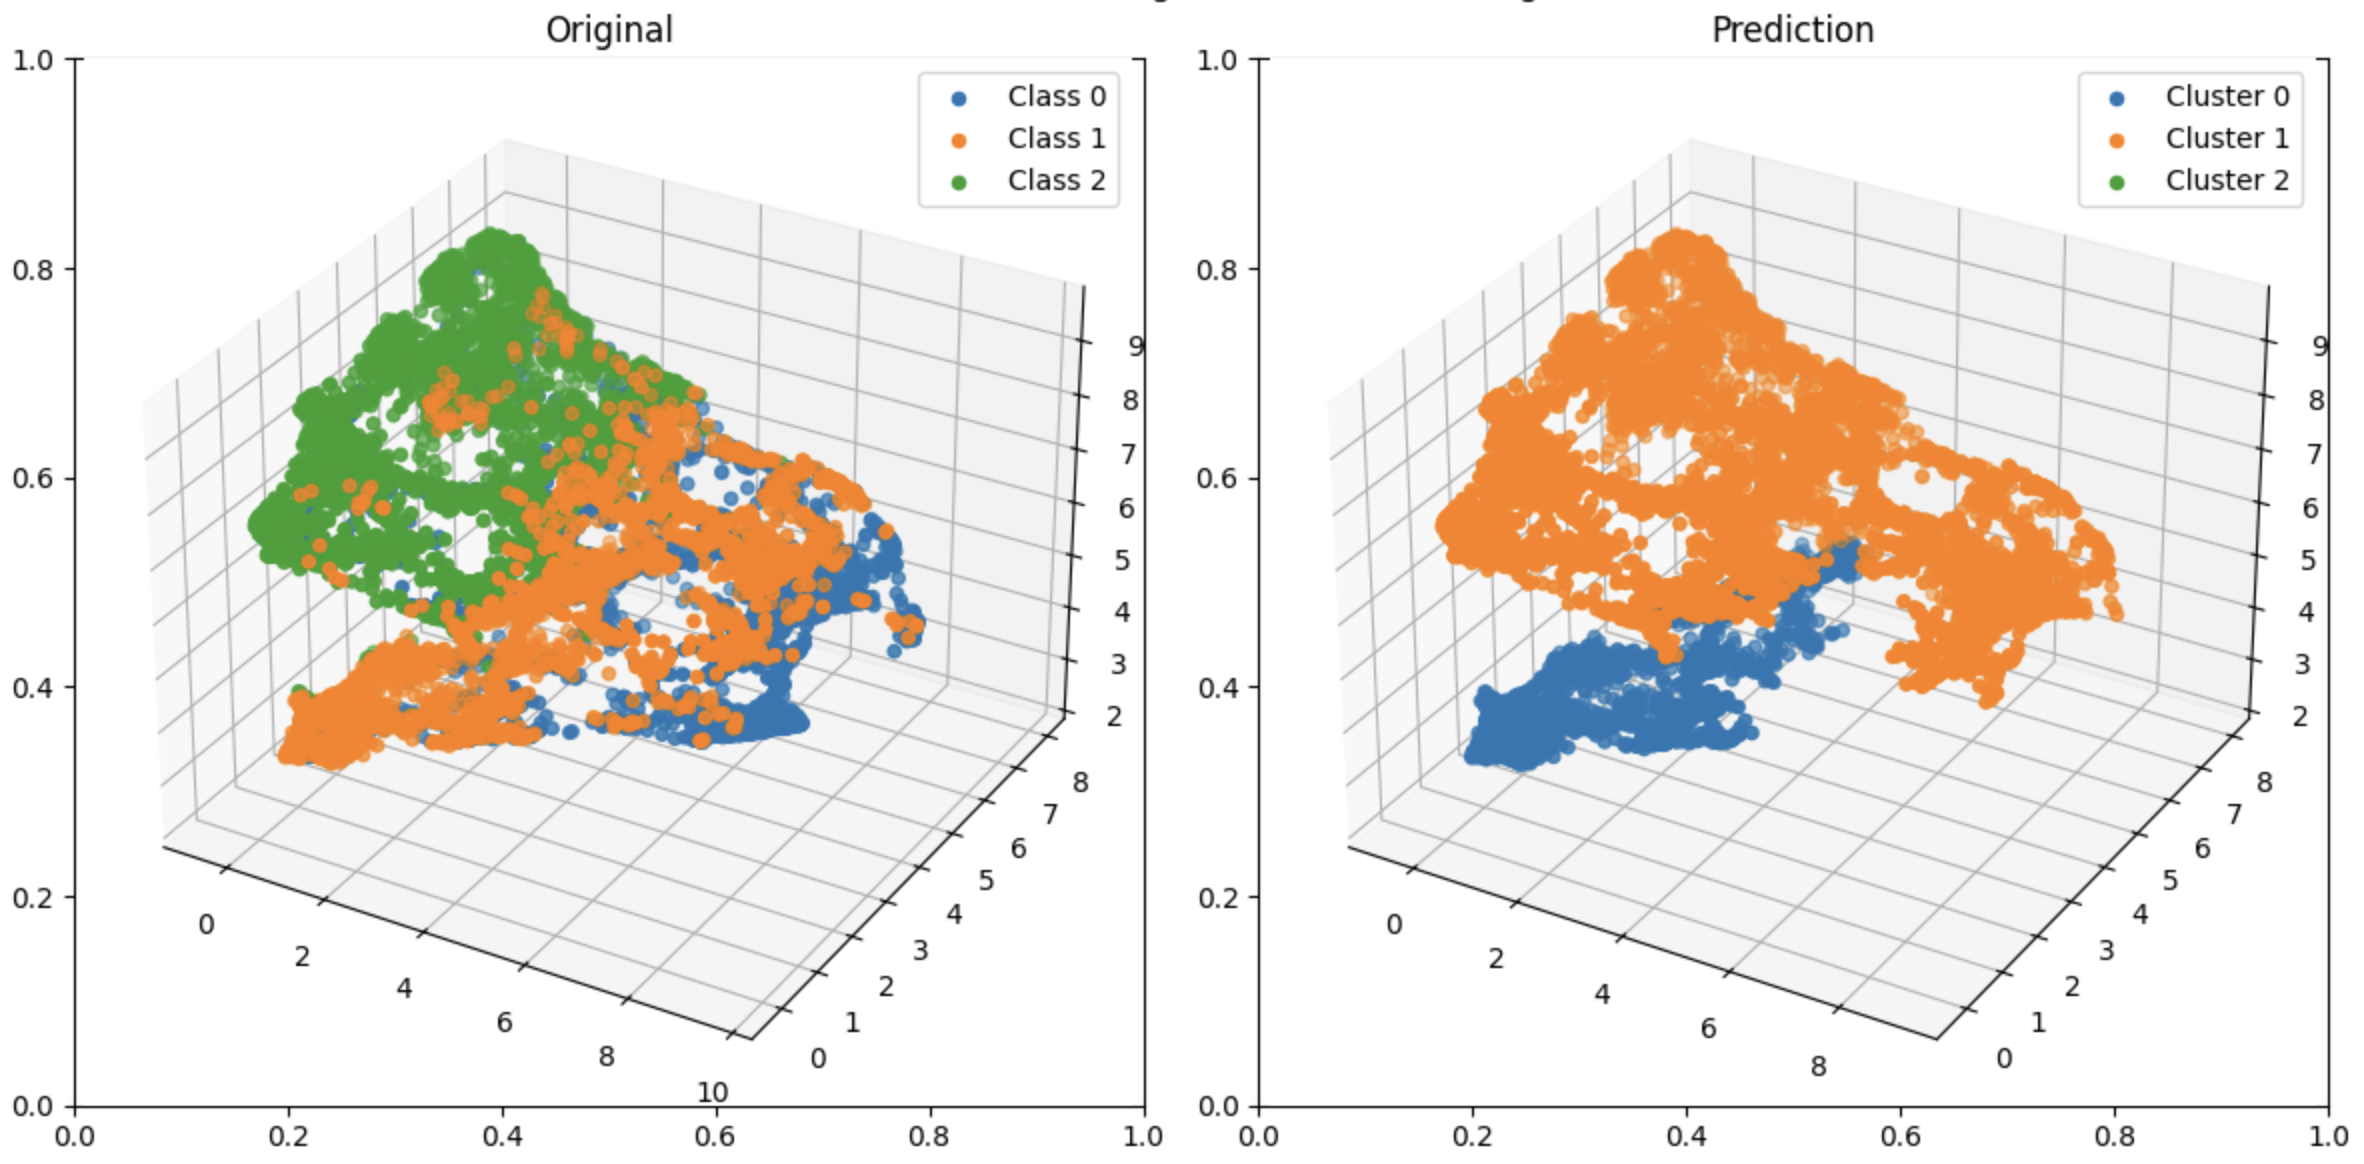
\includegraphics[width=\textwidth]{images/14.png}
	\end{center}
	\caption{Сравнение оригинального разбиения респондентов по укрупнённой шкале Кантрила с результатом кластеризации векторов, полученных после снижения размерности исходных данных с помощью алгоритма UMAP (ARI: 0.24)}
	\label{img:12}
\end{figure}

\begin{figure}
	\begin{center}
		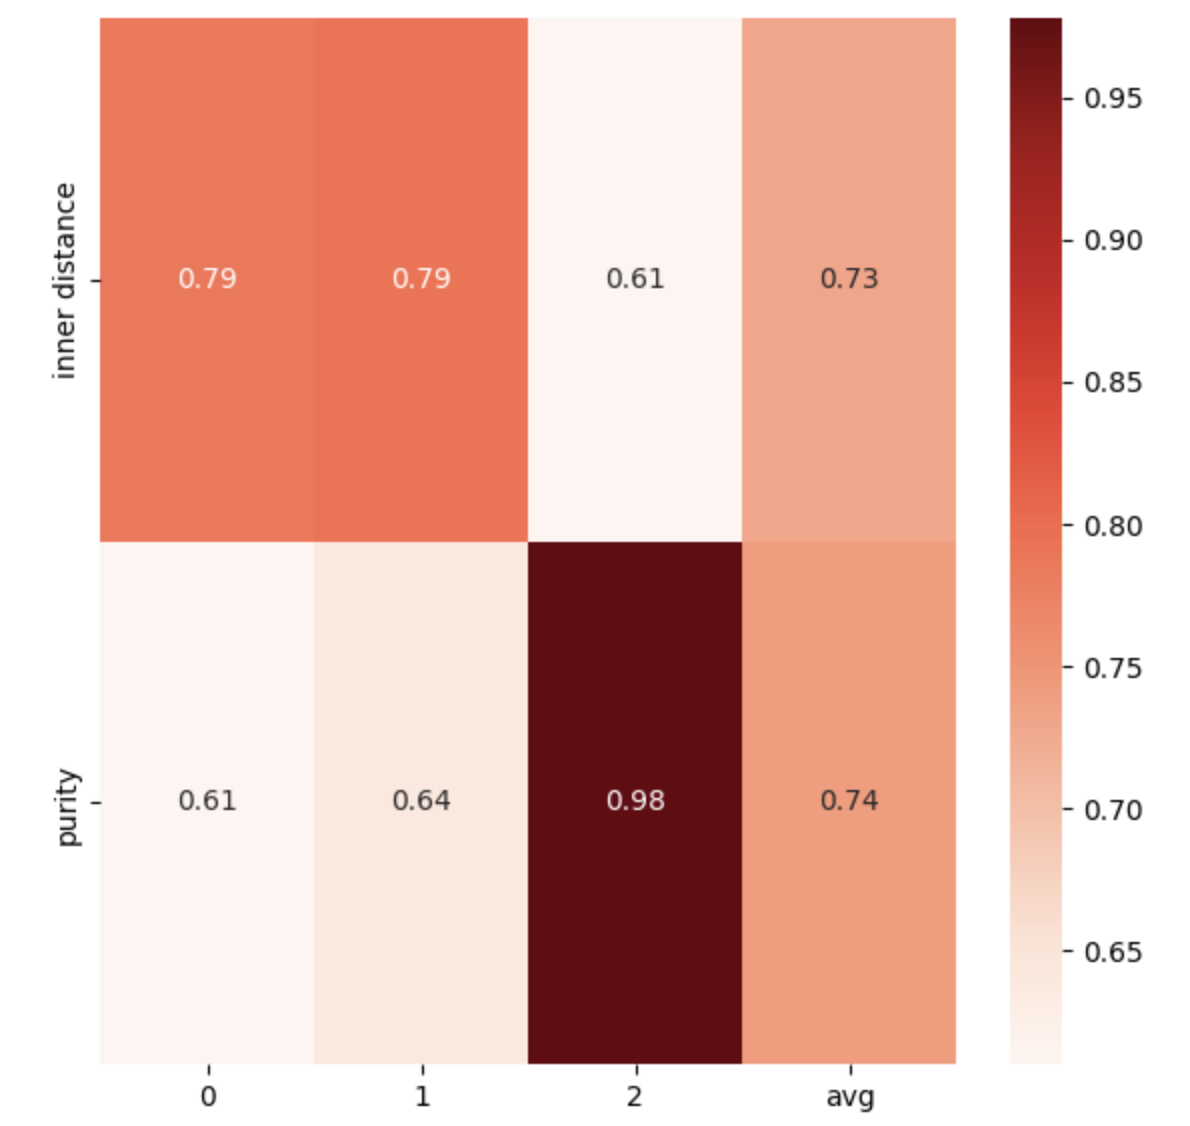
\includegraphics[width=0.65\textwidth]{images/16.png}
	\end{center}
	\caption{Соотнесение внутрикластерных расстояний с чистотой исходных кластеров, отсортированных по укрупнённой шкале Кантрила)}
	\label{img:13}
\end{figure}

\FloatBarrier

\subsection{Оптимизация гиперпараметров по метрике DBI}

\begin{figure}
	\begin{center}
		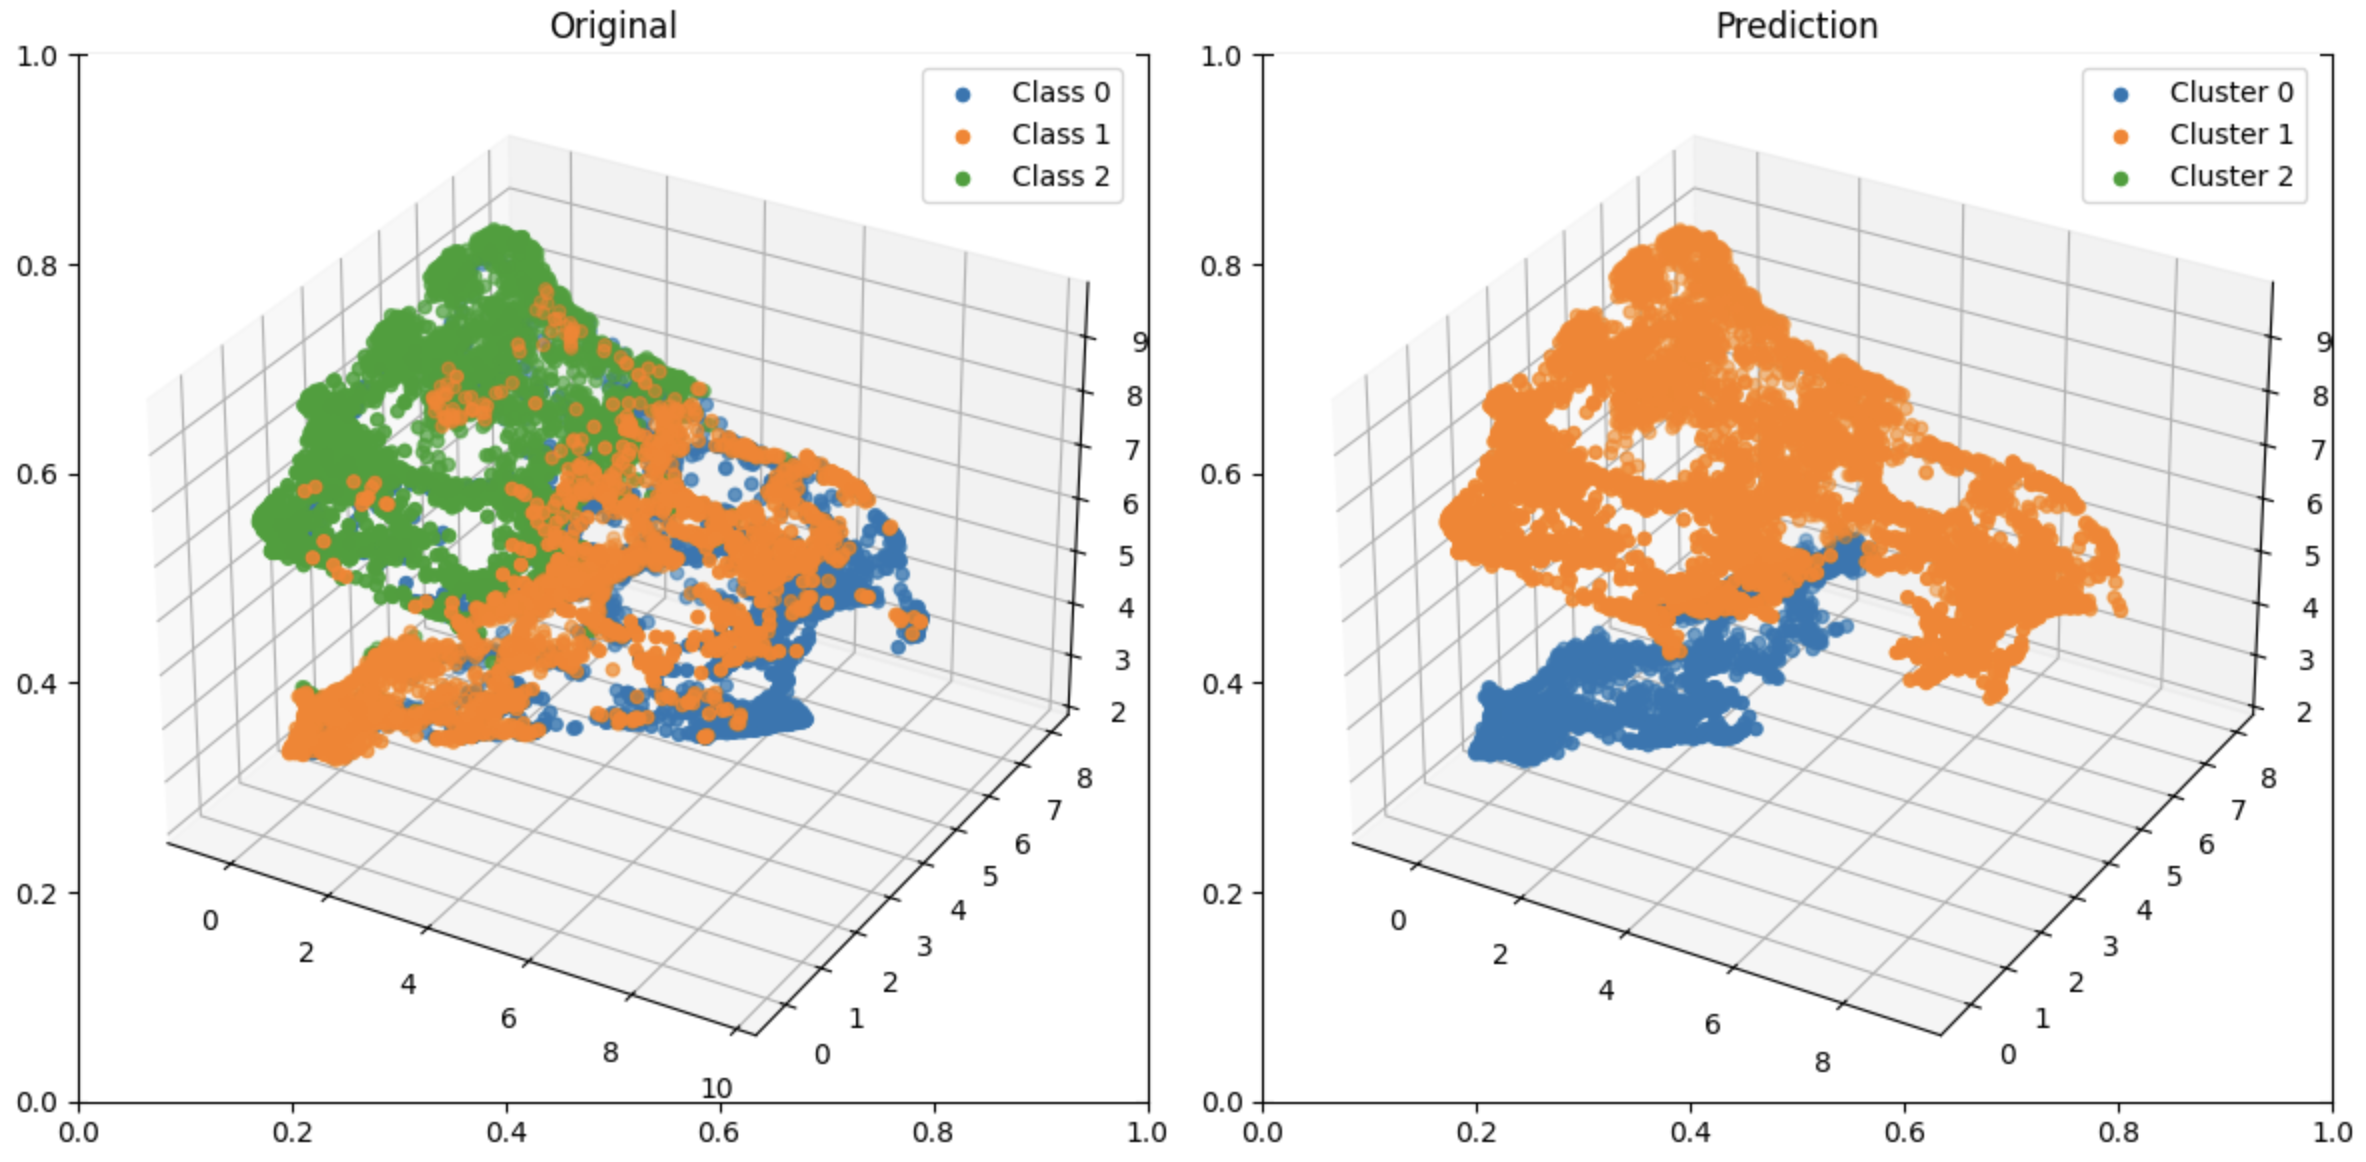
\includegraphics[width=\textwidth]{images/17.png}
	\end{center}
	\caption{Сравнение оригинального разбиения респондентов по укрупнённой шкале Кантрила с результатом кластеризации векторов, полученных после снижения размерности исходных данных с помощью алгоритма UMAP (ARI: 0.24)}
	\label{img:14}
\end{figure}

\begin{figure}
	\begin{center}
		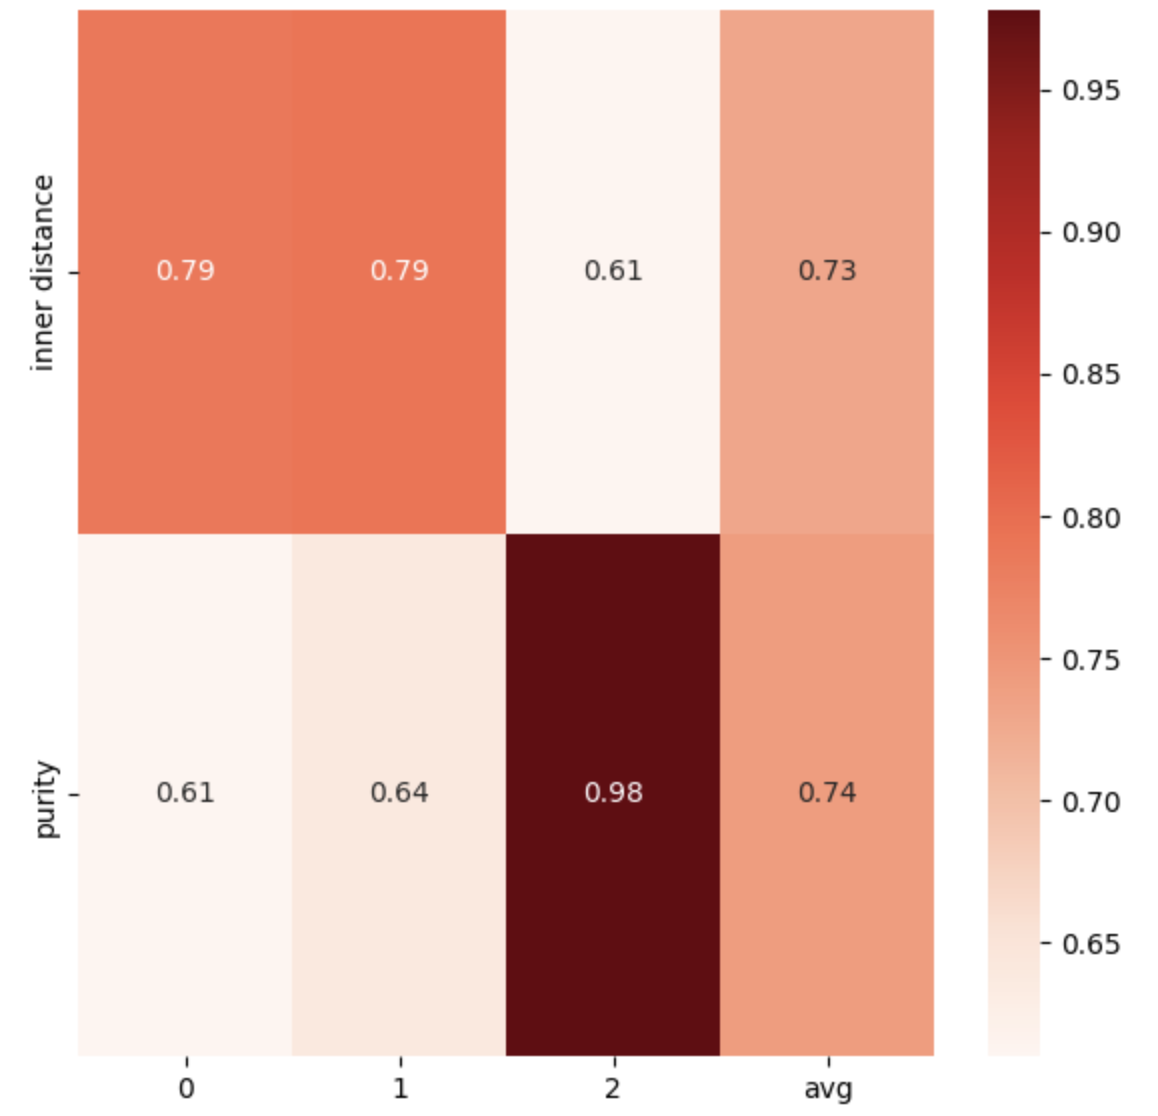
\includegraphics[width=0.65\textwidth]{images/18.png}
	\end{center}
	\caption{Соотнесение внутрикластерных расстояний с чистотой исходных кластеров, отсортированных по укрупнённой шкале Кантрила)}
	\label{img:15}
\end{figure}

\FloatBarrier
